\section{Durchführung}
\label{sec:Durchführung}
Die verwendete Schaltung und der Aufbau der Messapparatur ist in \ref{fig:schaltung} skizziert.

\begin{figure}
  \centering
  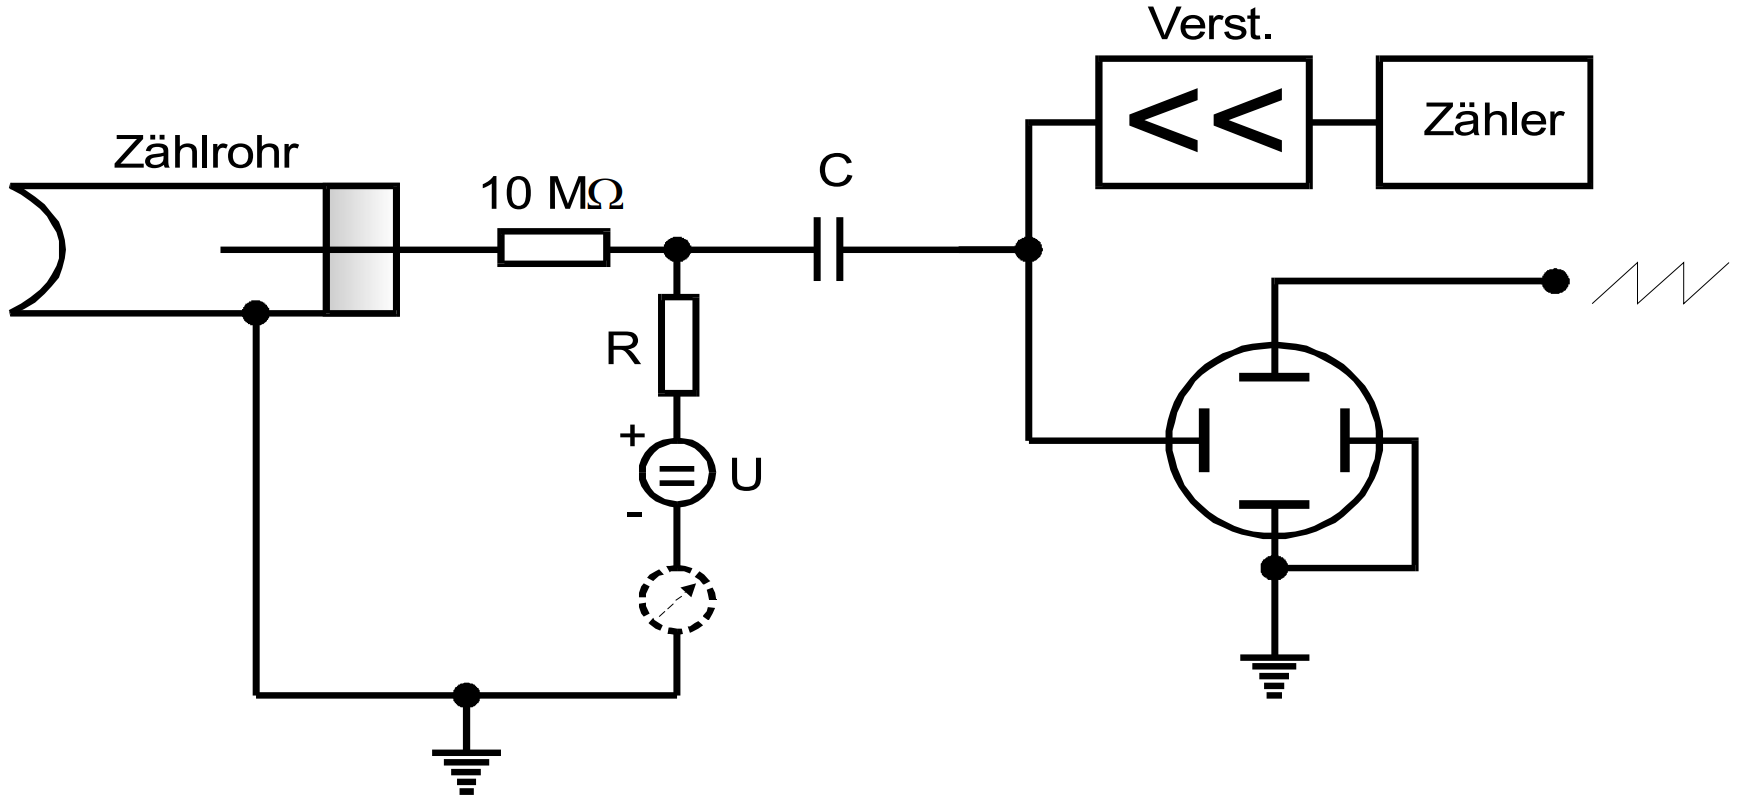
\includegraphics[width=\textwidth]{data/schaltung.png}
  \caption{Schaltbild und Aufbau der Apparatur,\cite{Versuchsanleitung}.}
  \label{fig:schaltung}
\end{figure}

Die am Draht aufgesammelte Ladung $Q$ resultiert in einem Strom, der über den Widerstand $R$
abfließt. Dadurch wird eine Spannung erzeugt, sodass ein Spannungsimpuls über den Kondensator
ausgekoppelt wird. Die Impulse werden verstärkt und dann gezählt. Außerdem können sie an einem Oszilloskop
beobachtet werden.\\
Es wird eine Betastrahlungsquelle vor das Fenster des Zählrohrs platziert.
Zunächst wird eine Messreihe der registrierten Ereignisse $N$ in einer Zeit von $t=\SI{60}{\second}$
in Abhängigkeit der anliegenden Spannung $U$ aufgenommen. Außerdem wird der durch die elektrischen
Impulse fließende Strom für jeden Spannungswert notiert. Der Messbereich erstreckt sich
von 300\,V bis 700\,V und es wird in Abständen von 10\,V gemessen.\\
Es wird eine Spannung von 400\,V eingestellt und der Verlauf der elektrischen Impulse
am Oszilloskop beobachtet. Dann wird unter Kenntnis der Ablenkgeschwindigkeit die Totzeit
abgelesen. Das ist gerade die Zeit, wenn sich der Triggerwert das erste Mal wiederholt.
Die weiteren Impulse flackern nach dem primären Impuls auf und sind zunächst noch niedriger
als der erste. Die Erholungszeit kann dann ungefähr als die Zeit abgeschätzt werden,
nachdem die Impulse ungefähr wieder die Höhe des ersten Impulses erreicht haben.\\
Zuletzt wird die Zwei-Qullen-Methode verwendet. Dabei wird zunächst die Zählrate $N_1$ gemessen,
wenn sich Quelle eins vor dem Zählrohr befindet. Danach wird Quelle zwei dazu gestellt und
die Zählrate $N_{1+2}$ gemessen. Daraufhin wird Quelle eins entfernt und die Zählrate $N_2$ gemessen.
